\documentclass[letterpaper,  %a4paper
               %boxit,
               %titlepage,   % separate title page
               %refpage      % separate references
              ]{jacow-2_3}   %jacow}
%
% CHANGE SEQUENCE OF GRAPHICS EXTENSION TO BE EMBEDDED
% ----------------------------------------------------
% test for XeTeX where the sequence is by default eps-> pdf, jpg, png, pdf, ...
%    and the JACoW template provides JACpic2v3.eps and JACpic2v3.jpg which
%    might generates errors, therefore PNG and JPG first
%
\makeatletter%
	\ifboolexpr{bool{xetex}}
	 {\renewcommand{\Gin@extensions}{.pdf,%
	                    .png,.jpg,.bmp,.pict,.tif,.psd,.mac,.sga,.tga,.gif,%
	                    .eps,.ps,%
	                    }}{}
\makeatother

% CHECK FOR XeTeX/LuaTeX BEFORE DEFINING AN INPUT ENCODING
% --------------------------------------------------------
%   utf8  is default for XeTeX/LuaTeX 
%   utf8  in LaTeX only realizes a small portion of codes
%
\ifboolexpr{bool{xetex} or bool{luatex}} % test for XeTeX/LuaTeX
 {}                                      % input encoding is utf8 by default
 {\usepackage[utf8]{inputenc}}           % switch to utf8

\usepackage[USenglish]{babel}			 

\usepackage[final]{pdfpages}
\usepackage{multirow}
\usepackage{ragged2e}
\usepackage{tikz}
\usetikzlibrary{shapes,arrows,snakes,backgrounds}
\usetikzlibrary{mindmap,trees}
\usetikzlibrary{decorations.pathreplacing}
\usetikzlibrary{plotmarks}
%
% if BibLaTeX is used
%
\ifboolexpr{bool{jacowbiblatex}}%
 {%
  \addbibresource{jacow-test.bib}
  \addbibresource{biblatex-examples.bib}
 }{}
\listfiles

%
% command for typesetting a \section like word
%
\newcommand\SEC[1]{\textbf{\uppercase{#1}}}

%%
%%   Lengths for the spaces in the title
%%   \setlength\titleblockstartskip{..}  %before title, default 3pt
%%   \setlength\titleblockmiddleskip{..} %between title + author, default 1em
%%   \setlength\titleblockendskip{..}    %afterauthor, default 1em

%\copyrightspace %default 1cm. arbitrary size with e.g. \copyrightspace[2cm]

% testing to fill the copyright space
%\usepackage{eso-pic}
%\AddToShipoutPictureFG*{\AtTextLowerLeft{\textcolor{red}{COPYRIGHTSPACE}}}

\begin{document}

\title{Staged Two Beam Acceleration Beam Line Design for the AWA Facility}

\author{N. Neveu\thanks{nneveu@anl.gov}\textsuperscript{1}, 
	    L. Spentzouris, Illinois Institute of Technology, Chicago, USA \\
	    J. G. Power, \textsuperscript{1}Argonne National Laboratory, Lemont, USA \\
	    C. Jing, Euclid Techlabs, Solon, Ohio, USA}
\maketitle

%
\begin{abstract}
Two beam acceleration is a candidate for future high energy physics machines and FEL user facilities. This scheme consists of two independent electron
beam lines operating synchronously. High-charge, 70 MeV drive bunch trains are injected from the RF photo-injector into decelerating structures to
generate a few hundred of MW of RF power. This RF power is transferred through an RF waveguide to accelerating structures that are used to
accelerate the witness beam. Staging refers to the sequential acceleration (energy gain) in two or more structures on the witness beam line. A kicker
was incorporated on the drive beam line to accomplish a modular design so that each accelerating structure can be independently powered by a
separate drive beam. Simulations were performed in OPAL-T to model the two beam lines. Beam sizes at the center of the structures was minimized to
ensure good charge transmission. Dispersion was minimized for bunches traveling through the kicker and dipoles. The resulting design will be the basis
for proof of principle experiments that will take place at the Argonne Wakefield Accelerator (AWA) facility.
\end{abstract}


\section{AWA Facility}
The AWA Facility houses two rf photoinjectors, both 
operating at \SI{1.3}{GHz}. The photoinjector used for 
these studies consists of a gun and solenoids followed
by six accelerating cavities, as shown in Fig.~\ref{beamline}. 
This beam line is capable of low (\SI{0.1}{nC}) and 
high charge (\SI{100}{nC}) operation. The bunch charge is 
routinely adjusted for depending on the requirements 
of the experiments downstream of the photoinjector.
Typical operating charges are 1, 4, 10, and \SI{40}{nC}. 
While these are the most
common operating modes, other charges have been requested 
and provided depending on the experiment.
Recent experiments include emittance exchange \cite{eex}, 
structure tests \cite{pets}, thermal emittance measurements \cite{therm}, 
and two beam acceleration \cite{tba}. 


\section{Kicker Tests}


\section{Simulations}
Simulations of the AWA beam line shown in Fig~\ref{beamline}
were performed in the PIC codes IMPACT~\cite{impact} and OPAL~\cite{opal}.
The gun, accelerating cavities, and solenoids were modeled with 2D
Poisson/Superfish~\cite{fish} files. All field maps were in the T7 format.
Input parameters for the simulations are shown in Table~\ref{simparam}.
Note that on crest refers to the phase of max energy gain.
In the case of the gun, a -~$20^{\circ}$ phase is measured 
w.r.t the phase of max energy gain. 
In other words, we ran $-20^{\circ}$ off crest.

\begin{figure*}[!tbh]
	\centering
	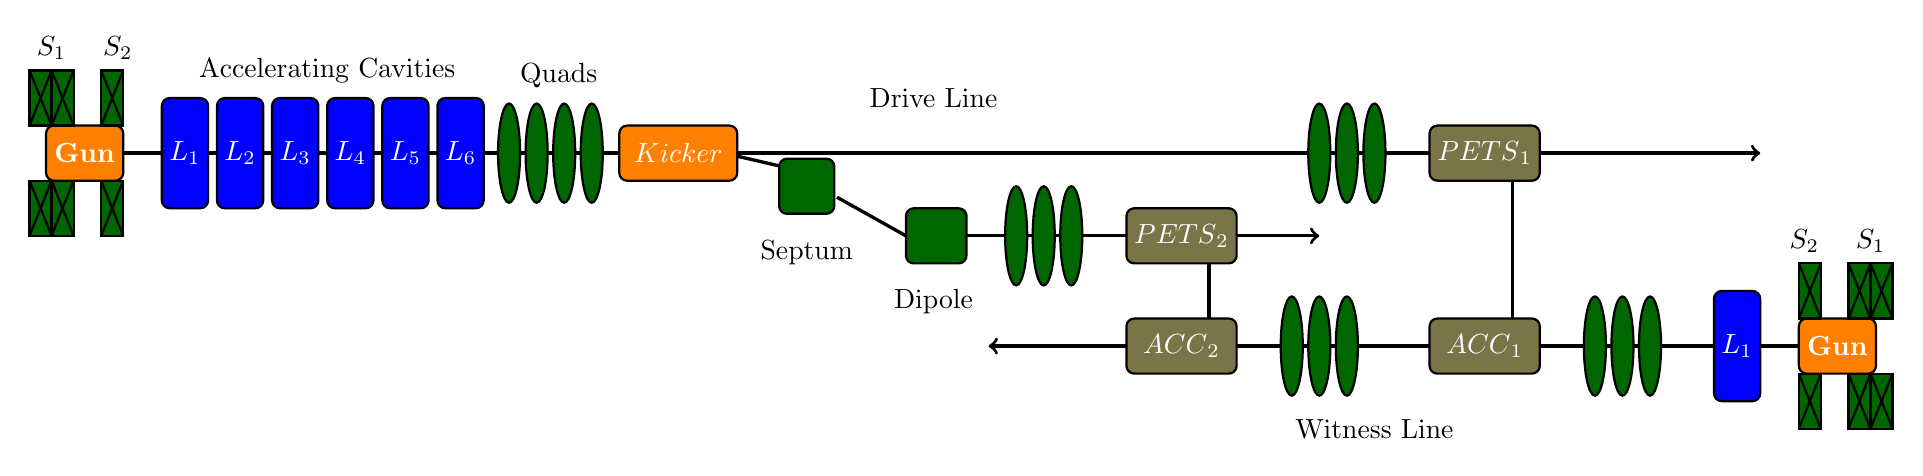
\begin{tikzpicture}[scale=0.7, text=black]
	\def \gunleft {-1.0}
\def \gunright {0.3}
\def \loneright {1.0}
\def \ltworight {2.0}
\def \lthreeright {3.0}
\def \lfourright {4.0}
\def \lfiveright {5.0}
\def \lsixright {6.0}
\def \quadone {7.3}
\def \quadfour{16}

\draw[very thick, ->] (0.0,1) -- (30,1);

\draw[fill=orange, thick, rounded corners =0.1cm] (\gunleft-0.1,0.5)rectangle (\gunright,1.5) node[pos=.5, white] {\textbf{Gun}} ;
%Straight through

%S1
\node[] at (-1,2.9) {$S_1$};
\draw[thick, fill=black!60!green] (-1.4,-0.5)rectangle  (-1.0,0.5) node[pos=.5, white] {} ;
\draw[black,  thick] (-1.4,-0.5) -- (-1.0,0.5);
\draw[black,  thick] (-1.4,0.5) -- (-1.0,-0.5);
\draw[ thick, fill=black!60!green] (-1.4,1.5)rectangle  (-1.0,2.5) node[pos=.5, white] {} ;
\draw[black,  thick] (-1.4,1.5) -- (-1.0,2.5);
\draw[black,  thick] (-1.4,2.5) -- (-1.0,1.5);

\draw[ thick, fill=black!60!green] (-1.0,-0.5)rectangle  (-0.6,0.5) node[pos=.5, white] {} ;
\draw[black,  thick] (-1.0,-0.5) -- (-0.6,0.5);
\draw[black,  thick] (-1.0,0.5) -- (-0.6,-0.5);
\draw[ thick, fill=black!60!green] (-1.0,1.5)rectangle  (-0.6,2.5) node[pos=.5, white] {} ;
\draw[black,  thick] (-1.0,1.5) -- (-0.6,2.5);
\draw[black,  thick] (-1.0,2.5) -- (-0.6,1.5);

%S2
\node[] at (0.2,2.9) {$S_2$};
\draw[ thick, fill=black!60!green] (-0.1,-0.5) rectangle  (0.3,0.5) node[pos=.5, white] {};
\draw[black,  thick] (-0.1,-0.5) -- (0.3,0.5);
\draw[black,  thick] (-0.1,0.5) -- (0.3,-0.5);
\draw[ thick, fill=black!60!green] (-0.1,1.5) rectangle  (0.3,2.5) node[pos=.5, white] {};
\draw[black,  thick] (-0.1,1.5) -- (0.3,2.5);
\draw[black,  thick] (-0.1,2.5) -- (0.3,1.5);
%Linac drawings 
\node[] at (4,2.5) {Accelerating Cavities};
\draw[fill=blue,  thick, rounded corners =0.1cm] (\loneright,0)rectangle  ({\loneright+0.84},2) node[pos=.5, white] {$L_1$} ;
\draw[fill=blue,  thick, rounded corners =0.1cm] (\ltworight,0)rectangle  ({\ltworight+0.84},2) node[pos=.5, white] {$L_2$};
\draw[fill=blue,  thick, rounded corners =0.1cm] (\lthreeright,0)rectangle ({\lthreeright+0.84},2) node[pos=.5, white] {$L_3$};
\draw[fill=blue,  thick, rounded corners =0.1cm] (\lfourright,0)rectangle ({\lfourright+0.84},2) node[pos=.5, white] {$L_4$};
\draw[fill=blue,  thick, rounded corners =0.1cm] (\lfiveright,0)rectangle ({\lfiveright+0.84},2) node[pos=.5, white] {$L_5$};
\draw[fill=blue,  thick, rounded corners =0.1cm] (\lsixright,0)rectangle ({\lsixright+0.84},2) node[pos=.5, white] {$L_6$};

%current optimization point
%\node[draw, fill=yellow, star, star points=5, star point ratio=0.6, minimum size=0.1cm]
%at (12.5,1.0) {$z_1$};


%Quad drawings
\node[] at (8.2,2.4) {Quads};
\draw[fill=black!60!green,  thick] (\quadone, 1.0) ellipse (0.2cm and 0.9cm);
\draw[fill=black!60!green,  thick] (\quadone+0.5, 1.0) ellipse (0.2cm and 0.9cm);
\draw[fill=black!60!green,  thick] (\quadone+1.0, 1.0) ellipse (0.2cm and 0.9cm);
\draw[fill=black!60!green,  thick] (\quadone+1.5, 1.0) ellipse (0.2cm and 0.9cm);

%Line between kicker and septum
\node[] at (15,2) {Drive Line};
\node[] at (23,-4) {Witness Line};
\draw[very thick] (\lsixright+5.2,1.0) -- (12.5,0.7);

%Kicker 
\draw[fill=orange,  thick, rounded corners =0.1cm] (\lsixright+3.3,0.5)rectangle ({\lsixright+0.84+4.6},1.5) node[pos=.5, white] {$Kicker$};

%Septum
\node[] at (12.7,-0.8) {Septum};
\draw[fill=black!60!green,  thick, rounded corners =0.1cm] (12.2,0.9)rectangle ({13.2},-0.1) node[pos=.5, white] {};
%\draw[latex-latex] (\gunleft,-5.0) -- (14,-5.0) ;
%\foreach \x in  {0.3, 1.0, 3.5, 5.0, 7.0, 8.5, 10, 12.5} %tick marks
%\draw[shift={(\x,-5.0)},color=black] (0pt,3pt) -- (0pt,-3pt);
%\foreach \x in {0.3, 1.0, 3.5, 5.0, 7.0, 8.5, 10, 12.5}
%\draw[shift={(\x,-5.2)},color=black] (0pt,0pt) node[below] {$\x$};

%Line between kicker and septum
\draw[very thick] (13.25,0.2) -- (14.5,-0.5);

%Dipole
\node[] at (15,-1.7) {Dipole};
\draw[fill=black!60!green, thick, rounded corners =0.1cm] (14.5,0.0)rectangle ({15.6},-1.0) node[pos=.5, white] {};

%Line between dipole and quads
\draw[very thick, ->] (15.6,-0.5) -- (22,-0.5);
%Second set of quads
\draw[fill=black!60!green,  thick] (\quadfour+0.5, -0.50) ellipse (0.2cm and 0.9cm);
\draw[fill=black!60!green,  thick] (\quadfour+1.0, -0.50) ellipse (0.2cm and 0.9cm);
\draw[fill=black!60!green,  thick] (\quadfour+1.5, -0.50) ellipse (0.2cm and 0.9cm);



\def \quadfive{22}
%Third set of quads
\draw[fill=black!60!green,  thick] (\quadfive, 1.0) ellipse (0.2cm and 0.9cm);
\draw[fill=black!60!green,  thick] (\quadfive+0.5, 1.0) ellipse (0.2cm and 0.9cm);
\draw[fill=black!60!green,  thick] (\quadfive+1.0, 1.0) ellipse (0.2cm and 0.9cm);


%Witness
\draw[very thick, <-] (16,-2.5) -- (31,-2.5);

%Waveguide
\draw[very thick] (20,-0.5) -- (20,-3);
%Waveguide
\draw[very thick] (25.5,1.5) -- (25.5,-3);

%PETS2
\draw[fill=black!60!yellow,  thick, rounded corners =0.1cm] (18.5,0.0)rectangle (20.5,-1) node[pos=.5, white] {$\text{PETS}_2$};
%PETS1
\draw[fill=black!60!yellow,  thick, rounded corners =0.1cm] (24,1.5)rectangle (26,0.5) node[pos=.5, white] {$\text{PETS}_1$};

%ACC2
\draw[fill=black!60!yellow,  thick, rounded corners =0.1cm] (18.5,-2)rectangle (20.5,-3) node[pos=.5, white] {$\text{ACC}_2$};
%ACC1
\draw[fill=black!60!yellow,  thick, rounded corners =0.1cm] (24,-2)rectangle (26,-3) node[pos=.5, white] {$\text{ACC}_1$};
\def \quadsix{27}
%Third set of quads
\draw[fill=black!60!green,  thick] (\quadsix, -2.5) ellipse (0.2cm and 0.9cm);
\draw[fill=black!60!green,  thick] (\quadsix+0.5, -2.5) ellipse (0.2cm and 0.9cm);
\draw[fill=black!60!green,  thick] (\quadsix+1.0, -2.5) ellipse (0.2cm and 0.9cm);
\def \quadseven{21.5}
%Third set of quads
\draw[fill=black!60!green,  thick] (\quadseven, -2.5) ellipse (0.2cm and 0.9cm);
\draw[fill=black!60!green,  thick] (\quadseven+0.5, -2.5) ellipse (0.2cm and 0.9cm);
\draw[fill=black!60!green,  thick] (\quadseven+1.0, -2.5) ellipse (0.2cm and 0.9cm);

\begin{scope}[yscale=1,xscale=-1, yshift=-3.5cm, xshift=-31cm]
	\draw[fill=orange, thick, rounded corners =0.1cm] (\gunleft-0.1,0.5)rectangle (\gunright,1.5) node[pos=.5, white] {\textbf{Gun}} ;
	
	%S1
	\node[] at (-1,2.9) {$S_1$};
	\draw[thick, fill=black!60!green] (-1.4,-0.5)rectangle  (-1.0,0.5) node[pos=.5, white] {} ;
	\draw[black,  thick] (-1.4,-0.5) -- (-1.0,0.5);
	\draw[black,  thick] (-1.4,0.5) -- (-1.0,-0.5);
	\draw[ thick, fill=black!60!green] (-1.4,1.5)rectangle  (-1.0,2.5) node[pos=.5, white] {} ;
	\draw[black,  thick] (-1.4,1.5) -- (-1.0,2.5);
	\draw[black,  thick] (-1.4,2.5) -- (-1.0,1.5);
	
	\draw[ thick, fill=black!60!green] (-1.0,-0.5)rectangle  (-0.6,0.5) node[pos=.5, white] {} ;
	\draw[black,  thick] (-1.0,-0.5) -- (-0.6,0.5);
	\draw[black,  thick] (-1.0,0.5) -- (-0.6,-0.5);
	\draw[ thick, fill=black!60!green] (-1.0,1.5)rectangle  (-0.6,2.5) node[pos=.5, white] {} ;
	\draw[black,  thick] (-1.0,1.5) -- (-0.6,2.5);
	\draw[black,  thick] (-1.0,2.5) -- (-0.6,1.5);
	
	%S2
	\node[] at (0.2,2.9) {$S_2$};
	\draw[ thick, fill=black!60!green] (-0.1,-0.5) rectangle  (0.3,0.5) node[pos=.5, white] {};
	\draw[black,  thick] (-0.1,-0.5) -- (0.3,0.5);
	\draw[black,  thick] (-0.1,0.5) -- (0.3,-0.5);
	\draw[ thick, fill=black!60!green] (-0.1,1.5) rectangle  (0.3,2.5) node[pos=.5, white] {};
	\draw[black,  thick] (-0.1,1.5) -- (0.3,2.5);
	\draw[black,  thick] (-0.1,2.5) -- (0.3,1.5);
	%Linac drawings 
	%\node[] at (4,2.5) {Accelerating Cavities};
	\draw[fill=blue,  thick, rounded corners =0.1cm] (\loneright,0)rectangle  ({\loneright+0.84},2) node[pos=.5, white] {$L_1$} ;
	
\end{scope}



	\end{tikzpicture}	
	\caption{TBA beam line layout at the AWA.}
	\label{beamline}
\end{figure*}


\begin{table}[hbt]
	%   \vspace*{-.5\baselineskip}
	\centering
	\caption{Simulation Parameters}
	\begin{tabular}{lcc}
		\toprule
		\textbf{Parameter} & \textbf{Low Charge}  & \textbf{High Charge} \\
		\midrule
		Charge       & \SI{1}{nC}        & \SI{40}{nC}    \\ %[3pt]
		Gun Gradient & \SI{65}{MV/m}     & \SI{65}{MV/m}  \\ %[3pt]
		Gun Phase    & \SI{-20}{}$^{\circ}$ & \SI{-20}{}$^{\circ}$ \\		 
		$S_1$        & \SI{500}{A}		 & \SI{500}{A}	  \\
		$S_2$		 & \SI{}{A}   	 & \SI{185}{A}		 \\
		Linac Phases & On crest          & On crest       \\
		Laser FWHM   & \SI{1.5}{ps}      & \SI{1.5}{ps}   \\ %[3pt]
		Laser Radius & \SI{2}{mm}        & \SI{9}{mm}     \\
		\bottomrule
	\end{tabular}
	\label{simparam}
	%   \vspace*{-\baselineskip}
\end{table}


\begin{figure}
	\begin{tikzpicture}[every node/.style={anchor=south west,inner sep=0pt},x=1mm, y=1mm,]   
	\node (fig1) at (0,0)
	{\includegraphics[width=0.5\textwidth]{kicker1}};
	\node[fill=white, inner sep=2pt] (txt2) at (35,15) {Interferometer};
	\node[fill=white, inner sep=2pt, rotate=26] (txt2) at (18,19.5) {Slit};	
	\node[fill=white, inner sep=2pt, rotate=20] (txt2) at (13,27) {Window};
	\end{tikzpicture}
	\caption{Interferometer used to capture CTR light as it exited a 
			window on the beam line. }
	\label{inter}
\end{figure}



\begin{figure}
	\begin{tikzpicture}[every node/.style={anchor=south west,inner sep=0pt},x=1mm, y=1mm,]   
	\node (fig1) at (0,0)
	{\includegraphics[width=0.5\textwidth]{kicker1}};
	\node[fill=white, inner sep=2pt] (txt2) at (35,8) {Interferometer};	
	\node[fill=white, inner sep=2pt] (txt2) at (55,25) {Window};	
	\node[fill=white, inner sep=2pt] (txt2) at (22,35) {Bolometer};
	\end{tikzpicture}
	\caption{Bolometer. }
	\label{bolo}
\end{figure}

\section{Data Analysis}
Give link to code used to find bunch length

\section{Results}
Compare simulations to experimental measurements
\begin{figure}[!htb]
	%   \vspace*{-.5\baselineskip}
	\centering
	%\includegraphics*[width=174pt]{JACpic_mc}
	\caption{Layout of papers.}
	\label{l2ea4-f1}
	%   \vspace*{-\baselineskip}
\end{figure}

\section{Conclusion}
Any conclusions should be in a separate section directly preceding
the \SEC{Acknowledgment}, \SEC{Appendix}, or \SEC{References} sections, in that
order.

\section{acknowledgments}
We also gratefully acknowledge the computing resources
provided on Bebop, a high-performance computing cluster
operated by the LCRC at Argonne National Laboratory.
This material is based upon work supported by the 
U.S. Department of Energy, Office of Science, under 
contract number DE-AC02-06CH11357 and grant number DE-SC0015479. 
Travel to IPAC'18 supported by the Division of Physics 
of the United States National Science Foundation 
Accelerator Science Program and the Division of 
Beam Physics of the American Physical Society.


\begin{thebibliography}{9}
\bibitem{eex}
G.~Ha \emph{et al.}, “Demonstration of Current Profile 
Shaping using Double Dog-Leg Emittance Exchange Beam 
Line at Argonne Wakefield Accelerator”
in \textit{Proc. IPAC’16}, 
Busan, South Korea, May 2016, 
paper TUOBB01.\\

\bibitem{pets}
J.~Shao \emph{et al.}, “PETS....”
in \textit{Proc. IPAC’18}, 
Vancouver, Canada, May 2018, 
paper xxx.\\

\bibitem{therm}
L.~Zheng \emph{et al.}, “Measurements of Thermal Emittance 
for Cesium Telluride Photocathodes in an L-Band RF Gun”
in \textit{Proc. IPAC’17}, 
Copenhagen, Denmark, May 2017, 
paper TUPAB074.\\

\bibitem{tba}
J.~Shao \emph{et al.}, “Recent Two-Beam 
Acceleration Activities at Argonne Wakefield Accelerator Facility”
in \textit{Proc. IPAC’17}, 
Copenhagen, Denmark, May 2017, 
paper WEPVA022.\\

\bibitem{ctr}
A.~Alpha \emph{et al.}, 
“A fascinating paper about CTR,”
in \emph{Proc. FEL’13}, 
New York, NY, USA, Aug. 2013, 
paper WEP033, pp. 27--29.\\

\bibitem{impact}
J.~Qiang \emph{et al.},
“...,”
, California, USA,
Rep. xxxx, 20xx-20xx.

\bibitem{opal}
A.~Adelmann \emph{et al.},
“The OPAL (Object Oriented Parallel Accelerator Library) framework,”
PSI, Zurich, Switzerland,
Rep. PSI-PR-08-02, 2008-2017.

\bibitem{fish}
\emph{Reference Manual for the POISSON/SUPERFISH Group of 
	Codes},  Los Alamos Accelerator Code Group,  
 Los Alamos, NM, USA, 
 Rep. LA-UR-87-126, Jan. 1987.
\end{thebibliography}




\end{document}
	
